\chapter{نتایج و تحلیل}
\label{ch:results}

در مجموع ۴۹ اجرای معتبر با مقیاس زمانی حقیقی انجام شد: چهار الگوی بار در برابر هفت بازوی
اصلی، به‌علاوه‌ی بازوهای حذفی و تکرارها. این فصل نتایج را گزارش و تحلیل می‌کند.

ترتیب ارائه از سطوح پایین‌تر ارزیابی به سطوح بالاتر می‌رود، سپس به نتیجه‌ی اصلی پروژه
می‌رسد، و در پایان بخشی مفصل به محدودیت‌های اعتبار اختصاص می‌یابد. آن بخش پایانی عمداً بلند
است: در جریان کار چند نقص اندازه‌گیری کشف شد که هیچ‌کدام را بررسی‌های خودکار
بخش~\ref{sec:method-validity} نگرفته بودند.

\section{آزمون‌های واحد}
\label{sec:results-unit}

منطق موتور سیاست مستقل از خوشه آزموده شد. پوشش آزمون به تفکیک بسته در
جدول~\ref{tab:results-coverage} آمده است.

\begin{table}[H]
\centering
\caption{پوشش آزمون به تفکیک بسته}
\label{tab:results-coverage}
\begin{tabular}{|l|r|p{6cm}|}
\hline
\textbf{بسته} & \textbf{پوشش} & \textbf{یادداشت} \\
\hline
\code{internal/policy} & \textbf{۹۹/۱ درصد} & ۴۵ آزمون، ۸۲ مورد با زیرآزمون‌ها \\
\code{internal/metrics} & ۸۵/۴ درصد & \\
\code{internal/config} & ۷۸/۴ درصد & \\
\code{internal/controller} & ۷۴/۶ درصد & \\
\code{internal/observability} & ۶۵/۱ درصد & \\
\code{internal/scaler} & ۵۹/۳ درصد & شکاف پوشش \code{restConfig} است که به خوشه‌ی زنده نیاز دارد \\
\code{cmd/*} & ۰ درصد & تنها سیم‌کشی مؤلفه‌ها \\
\hline
\end{tabular}
\end{table}

کف برنامه‌ریزی‌شده برای بسته‌ی \code{internal/policy} هشتاد درصد بود. در این بسته تنها یک
شاخه پوشش داده نشده است: حالت اشباع منفی در \code{ceilToReplicas}. این حالت از راه واسط عمومی
دست‌نیافتنی است، چون هر دو فراخواننده ورودی منفی و \lr{NaN} را پیش‌تر کنار می‌گذارند \mdash{} یعنی
همان نگهبانی که بخش~\ref{sec:design-defects} توصیف کرد، خودش دلیل پوشش‌نیافتن است.

مجموعه‌آزمون عمداً به شکل \textbf{مشخصه} نوشته شده و نه صرفاً به شکل نگهبان بازگشت. هر مورد،
ویژگی‌ای را که تثبیت می‌کند به‌صراحت نام می‌برد. پرسش‌هایی هم که داور احتمالاً می‌پرسد صریح و
یافتنی است: سقف‌گیری در برابر گردکردن، ناحیه‌ی مرده، صفر بودن نمونه‌های آماده، و مرز پنجره‌ی
۹۰ ثانیه‌ای.

مهم‌ترین آزمون این مجموعه از نظر علمی، \code{TestPerReplica\-Forecasting\-Oscillates\-Under\-ConstantLoad}
است که نتیجه‌اش در جدول~\ref{tab:design-oscillation-unit} آمد: زیر بار کل \emph{ثابت}، سیاست
درست صفر تغییر و سیاست معیوب ۲۹ تغییر در ۳۰ گام دارد. چون این آزمون هیچ زیرساختی ندارد، هیچ
توضیح رقیبی \mdash{} نویز شبکه، زمان‌بندی، تأخیر جمع‌آوری \mdash{} برای آن ۲۹ تغییر باقی نمی‌ماند.

\section{آزمون‌های یکپارچه‌سازی}
\label{sec:results-integration}

رفتار کل سامانه روی خوشه‌ی آزمایشی سنجیده شد: مقیاس‌گیری به بالا هنگام افزایش بار،
مقیاس‌گیری به پایین هنگام کاهش بار، و پایداری در برابر نوسان‌های کوتاه. سه مشاهده‌ی
یکپارچه‌سازی ارزش گزارش دارند.

\textbf{مقیاس‌گذار مالکیت تعداد نمونه را در دست دارد.} یک \lr{kubectl scale} دستی در چرخه‌ی
بعدی بازگردانده می‌شود. این رفتار درست است و نشان می‌دهد حلقه‌ی آشتی‌دهی واقعاً بسته است.

\textbf{سیاست پیش‌بینانه، پیش از رسیدن بار عمل می‌کند.} در یک اجرای واقعی، دنباله‌ی زیر از
گزارش‌های ساختاریافته‌ی خود مقیاس‌گذار بیرون آمد:

\begin{latin}
\begin{lstlisting}
 1 -> 2   ready=1  metric= 91.2  scale-up (immediate)
 2 -> 3   ready=2  metric= 75.1  scale-up (immediate)
 3 -> 4   ready=3  metric= 70.0  scale-up (immediate)
 4 -> 3   ready=4  metric= 54.6  scale-down (stabilized)
\end{lstlisting}
\end{latin}

سنجه‌ی مشاهده‌شده در \emph{هر} مقیاس‌گیری به بالا زیر نقطه‌ی هدف ۱۰۰ بود. ظرفیت افزوده شد چون
\emph{بار کل پیش‌بینی‌شده} در حال بالا رفتن بود: در آخرین نمونه،
\code{autoscaler\_predicted\_value} برابر ۲۲۱/۷ در برابر \code{autoscaler\_metric\_value}
برابر ۵۴/۶. یک سیاست واکنشی در هیچ‌یک از این سه لحظه حرکت نمی‌کرد. این، سیاست پیش‌بینانه است
که سیاست واکنشی را جلو می‌زند، و از گزارش‌های خود سامانه بیرون آمده است و نه از یک نمودار.

\textbf{بازوی \arm{hpa-custom} روی همان سیگنال کار می‌کند.} پیش از صرف دو ساعت زمان خوشه، با
عرضه‌ی ۹۰۰ درخواست بر ثانیه بررسی شد که واسط سنجه‌های سفارشی، ۸ نمونه از ۸ نمونه را با حدود
۱۱۲ درخواست بر ثانیه هر کدام گزارش می‌کند؛ یعنی تقسیم یکنواخت. این وارسی، پیش‌شرط اعتبار آن
بازو بود.

\section{نتایج مقایسه‌ای}
\label{sec:results-comparison}

\subsection{تصویر کلی}
\label{sec:results-headline}

جدول~\ref{tab:results-headline} سه سنجه‌ی اصلی را برای هر چهار الگوی بار کنار هم می‌گذارد.
جدول‌های کامل به تفکیک الگو، شامل همه‌ی ستون‌ها، در پیوست ج آمده است.

\begin{table}[H]
\centering
\small
\caption{نتایج اصلی؛ در هر الگو، کم‌ترین مقدار هر ستون \emph{در میان بازوهای خودکار} پررنگ
است. دو بازوی \arm{static} و \arm{static-peak} خط مبنا هستند و در این مقایسه وارد نمی‌شوند}
\label{tab:results-headline}
\begin{tabular}{|l|l|r|r|r|}
\hline
\textbf{بار کاری} & \textbf{بازو} & \textbf{نقض \lr{SLA}} & \textbf{نمونه-ثانیه} & \textbf{کم‌تأمین} \\
\hline
\arm{spike} & \arm{static-peak} & \lr{0.0\%} & \lr{23,530} & \lr{0} \\
\arm{spike} & \arm{static} & \lr{32.9\%} & \lr{14,480} & \lr{3,000} \\
\arm{spike} & \arm{hpa-cpu} & \lr{1.7\%} & \lr{13,915} & \lr{480} \\
\arm{spike} & \arm{hpa-custom} & \lr{2.2\%} & \lr{12,255} & \lr{475} \\
\arm{spike} & \arm{ours-threshold} & \lr{2.5\%} & \textbf{\lr{11,925}} & \lr{1,095} \\
\arm{spike} & \arm{ours-predictive} & \textbf{\lr{0.6\%}} & \lr{14,280} & \textbf{\lr{270}} \\
\hline
\arm{diurnal} & \arm{static-peak} & \lr{0.0\%} & \lr{21,720} & \lr{0} \\
\arm{diurnal} & \arm{static} & \lr{40.3\%} & \lr{14,480} & \lr{2,490} \\
\arm{diurnal} & \arm{hpa-cpu} & \textbf{\lr{0.0\%}} & \lr{15,570} & \lr{370} \\
\arm{diurnal} & \arm{hpa-custom} & \lr{4.7\%} & \textbf{\lr{14,365}} & \lr{1,070} \\
\arm{diurnal} & \arm{ours-threshold} & \lr{3.6\%} & \lr{14,545} & \lr{1,025} \\
\arm{diurnal} & \arm{ours-predictive} & \textbf{\lr{0.0\%}} & \lr{15,180} & \textbf{\lr{245}} \\
\hline
\arm{bursty} & \arm{static-peak} & \lr{0.0\%} & \lr{21,720} & \lr{0} \\
\arm{bursty} & \arm{static} & \lr{17.4\%} & \lr{14,480} & \lr{1,440} \\
\arm{bursty} & \arm{hpa-cpu} & \lr{2.5\%} & \lr{13,880} & \lr{1,200} \\
\arm{bursty} & \arm{hpa-custom} & \lr{4.4\%} & \textbf{\lr{11,965}} & \lr{1,260} \\
\arm{bursty} & \arm{ours-threshold} & \lr{3.3\%} & \lr{12,365} & \lr{1,410} \\
\arm{bursty} & \arm{ours-predictive} & \textbf{\lr{1.1\%}} & \lr{14,385} & \textbf{\lr{960}} \\
\hline
\arm{ramp} & \arm{static-peak} & \lr{0.0\%} & \lr{21,720} & \lr{0} \\
\arm{ramp} & \arm{static} & \lr{35.6\%} & \lr{14,480} & \lr{2,420} \\
\arm{ramp} & \arm{hpa-cpu} & \textbf{\lr{0.0\%}} & \lr{12,990} & \lr{605} \\
\arm{ramp} & \arm{hpa-custom} & \lr{4.7\%} & \lr{12,040} & \lr{1,230} \\
\arm{ramp} & \arm{ours-threshold} & \lr{4.1\%} & \textbf{\lr{11,810}} & \lr{1,460} \\
\arm{ramp} & \arm{ours-predictive} & \textbf{\lr{0.0\%}} & \lr{13,515} & \textbf{\lr{270}} \\
\hline
\end{tabular}
\end{table}

\textbf{در میان بازوهای خودکار، سیاست پیش‌بینانه روی هر چهار بار کاری کم‌ترین کم‌تأمین منابع
را دارد} (۲۷۰، ۲۴۵، ۹۶۰ و ۲۷۰ نمونه-ثانیه، در برابر کم‌ترین رقیب ۴۷۵، ۳۷۰، ۱۲۰۰ و ۶۰۵).
در نقض کیفیت خدمت روی \arm{spike} و \arm{bursty} کم‌ترین است و روی \arm{diurnal} و
\arm{ramp} با \arm{hpa-cpu} هم‌تراز؛ آنجا این ستون تفکیک نمی‌کند و تفکیک از کم‌تأمین منابع
و زمان واکنش می‌آید. خط مبنای ایستای \arm{static-peak} روی هر چهار الگو صفر و صفر است و
هیچ بازوی خودکاری بر آن غلبه نمی‌کند؛ بهای آن در ستون نمونه-ثانیه دیده می‌شود.

اما این برتری رایگان نیست: در هر چهار مورد، بازوی پیش‌بینانه از
\arm{hpa-custom} \emph{گران‌تر} است. آنچه سیاست پیش‌بینانه پیشنهاد می‌کند یک \textbf{مبادله}
است \mdash{} کیفیت خدمت و سرعت واکنش را می‌خرد و بهای آن را با ظرفیت بیشتر می‌پردازد. اندازه‌ی این
بها میان ۵/۷ تا ۲۰/۲ درصد نمونه-ثانیه است (نسبت به \arm{hpa-custom}: ۵/۷ درصد روی
\arm{diurnal}، ۱۲/۳ درصد روی \arm{ramp}، ۱۶/۵ درصد روی \arm{spike} و ۲۰/۲ درصد روی
\arm{bursty}).

نکته‌ی سومی هم در جدول هست که به‌آسانی از قلم می‌افتد: \arm{static-peak} همان ۰/۰ درصد نقض
\arm{ours-predictive} را دارد، اما روی \arm{ramp} با ۲۱،۷۲۰ نمونه-ثانیه در برابر ۱۳،۵۱۵،
یعنی \textbf{۶۱ درصد ظرفیت بیشتر برای نتیجه‌ی یکسان}. این، استدلال هزینه‌ای مقیاس‌گذاری
خودکار است و همان مقایسه‌ای است که وقتی تنها خط مبنای ایستا \arm{static} بود در دسترس نبود.

\subsection{تحلیل به تفکیک بار کاری}
\label{sec:results-perworkload}

شکل‌های~\ref{fig:cmp-diurnal} تا~\ref{fig:cmp-bursty} رفتار همه‌ی بازوها را در طول هر اجرا
نشان می‌دهند. هر شکل سه بخش دارد: بار عرضه‌شده در برابر بار اندازه‌گیری‌شده، تعداد نمونه‌های
آماده در برابر نیاز مرجع، و بار هر نمونه در برابر خط هدف و خط کیفیت خدمت.

\begin{figure}[H]
\centering
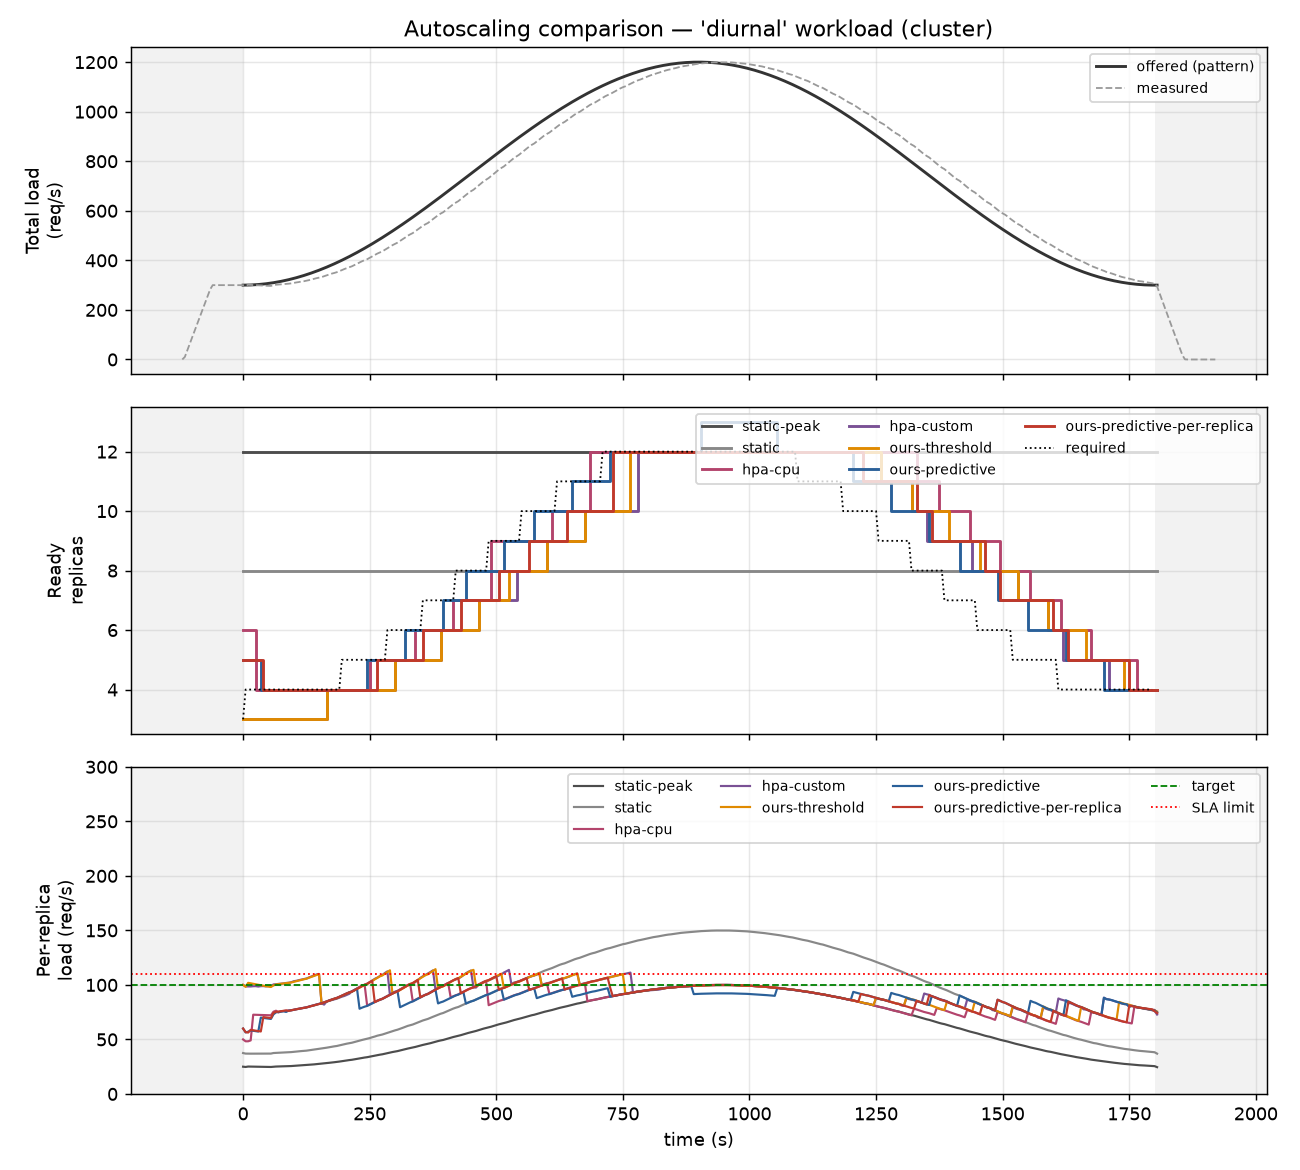
\includegraphics[width=\linewidth]{figures/comparison-diurnal.png}
\caption[مقایسه‌ی بازوها روی بار کاری \lr{diurnal}]{مقایسه‌ی بازوها روی \arm{diurnal}. نوار
خاکستری دو سو، مرحله‌های گرم‌کردن و نشست است و در محاسبه‌ی سنجه‌ها وارد نمی‌شود.}
\label{fig:cmp-diurnal}
\end{figure}

\textbf{\arm{ramp} (شکل~\ref{fig:cmp-ramp}): ستون نقض کیفیت خدمت تفکیک نمی‌کند و این باید
گفته شود.} چهار بازو از شش
بازو روی این الگو ۰/۰ درصد نقض دارند. علتش در خود الگو است: \arm{ramp} در بیست دقیقه ۱۰۰۰
درخواست بر ثانیه بالا می‌رود، یعنی حدود ۰/۸۳ درخواست بر ثانیه در هر ثانیه، یا تقریباً یک
نمونه‌ی اضافی در هر دو دقیقه. این آهنگ آن‌قدر آرام است که یک حلقه‌ی ۱۵ ثانیه‌ای با
راه‌اندازی ۳۰ ثانیه‌ای بتواند به‌صورت واکنشی آن را دنبال کند. ستون‌هایی که در اینجا تفکیک
می‌کنند، \emph{کم‌تأمین منابع} و \emph{زمان واکنش} هستند. گزارش کردن تنها ستون اشباع‌شده،
بازوها را غیرقابل‌تمایز نشان می‌داد در حالی که نیستند.

\begin{figure}[H]
\centering
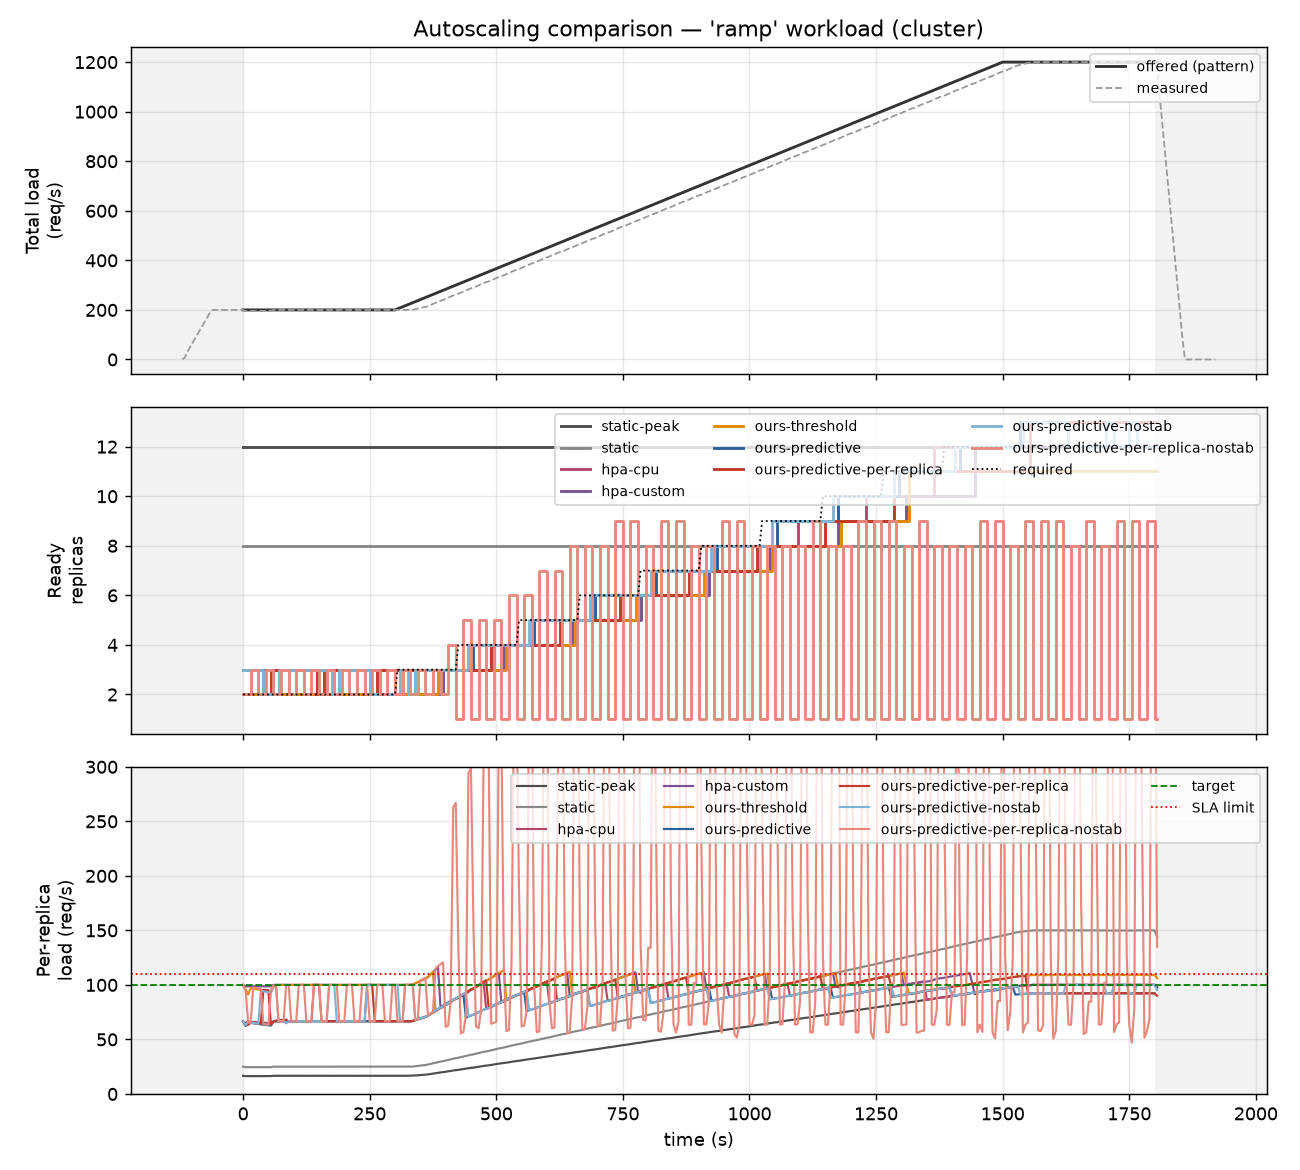
\includegraphics[width=\linewidth]{figures/comparison-ramp.png}
\caption[مقایسه‌ی بازوها روی بار کاری \lr{ramp}]{مقایسه‌ی بازوها روی \arm{ramp}. بازوی
\arm{ours-predictive-per-replica-nostab} ناوگان خود را تا یک نمونه فرو می‌پاشاند.}
\label{fig:cmp-ramp}
\end{figure}

\textbf{\arm{spike} (شکل~\ref{fig:cmp-spike}): نخستین بازوهایی که اصلاً زمان واکنش ندارند.} بازوهای \arm{static} و
\arm{ours-threshold} روی این الگو تا پایان پنجره هرگز به ۱۳ نمونه‌ی لازم نرسیدند. زمان واکنش
برای آن‌ها یک عدد گمشده نیست؛ \emph{خودِ نتیجه} است، و جدول باید آن را چنین بخواند و نه به
شکل خط تیره‌ای که ممکن است «آنی» فهمیده شود.

\begin{figure}[H]
\centering
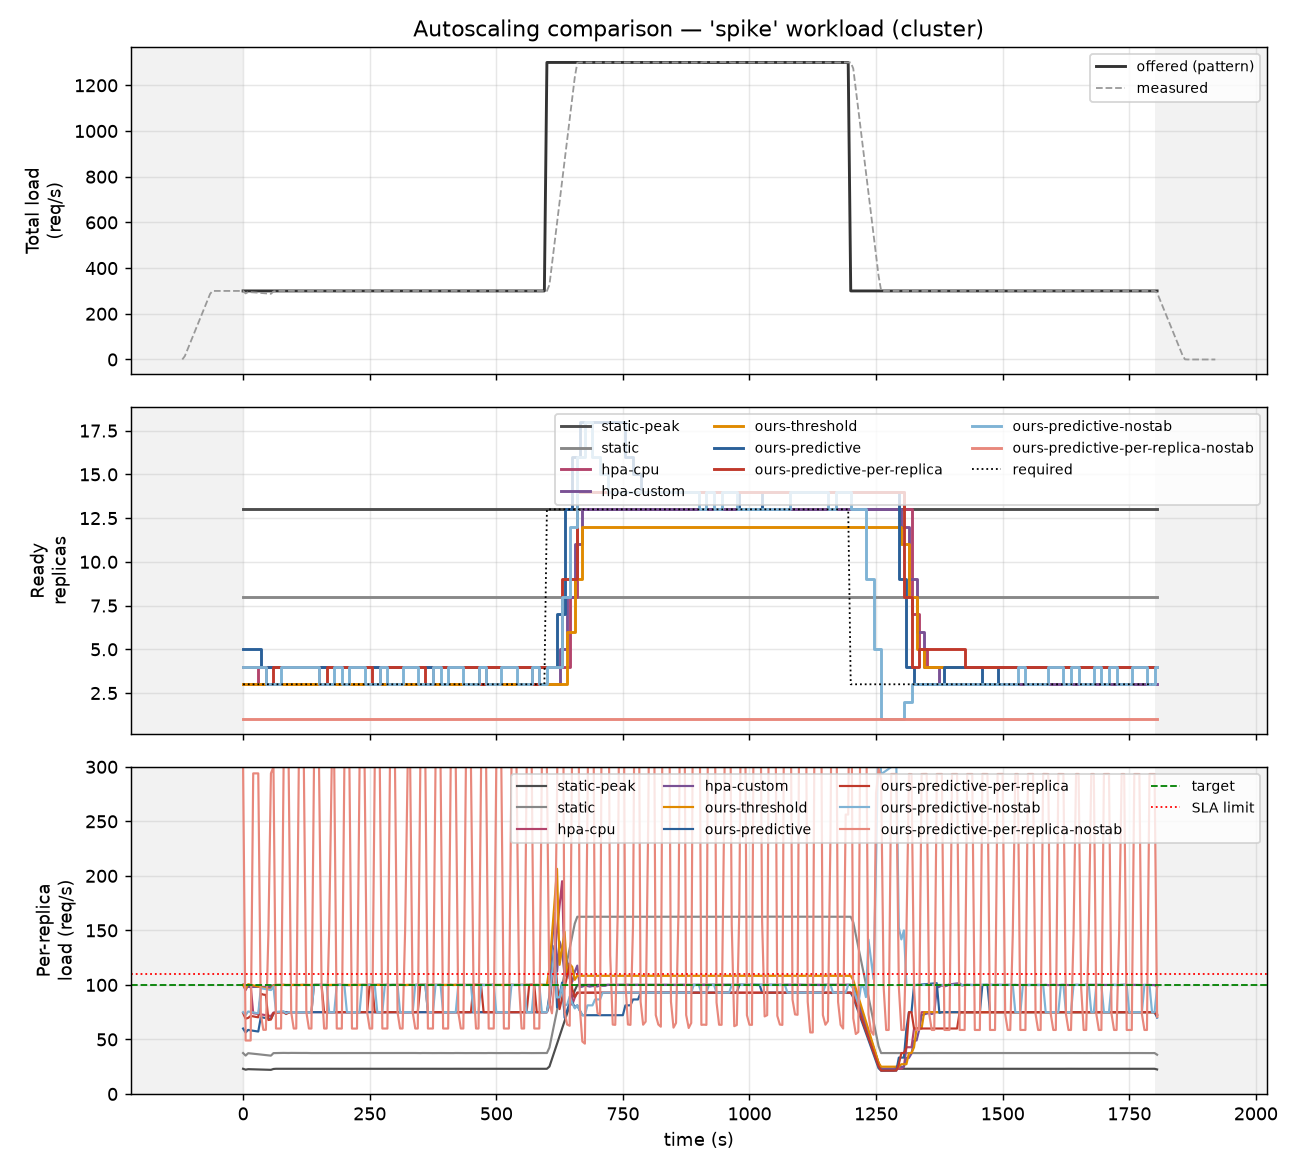
\includegraphics[width=\linewidth]{figures/comparison-spike.png}
\caption[مقایسه‌ی بازوها روی بار کاری \lr{spike}]{مقایسه‌ی بازوها روی \arm{spike}.}
\label{fig:cmp-spike}
\end{figure}

\textbf{\arm{diurnal} (شکل~\ref{fig:cmp-diurnal}): مقایسه‌ی «ارزش مقیاس‌گذاری» در تمیزترین
شکل خود.} روی این الگو
\arm{ours-threshold} با ۱۴،۵۴۵ نمونه-ثانیه در برابر ۱۴،۴۸۰ نمونه-ثانیه‌ی \arm{static} کار
می‌کند \mdash{} یعنی عملاً \emph{همان هزینه} \mdash{} و نقض کیفیت خدمت را از ۴۰/۳ درصد به ۳/۶ درصد
می‌رساند. روشن‌ترین بیان ارزش مقیاس‌گذاری خودکار در این مجموعه همین است.

\begin{figure}[H]
\centering
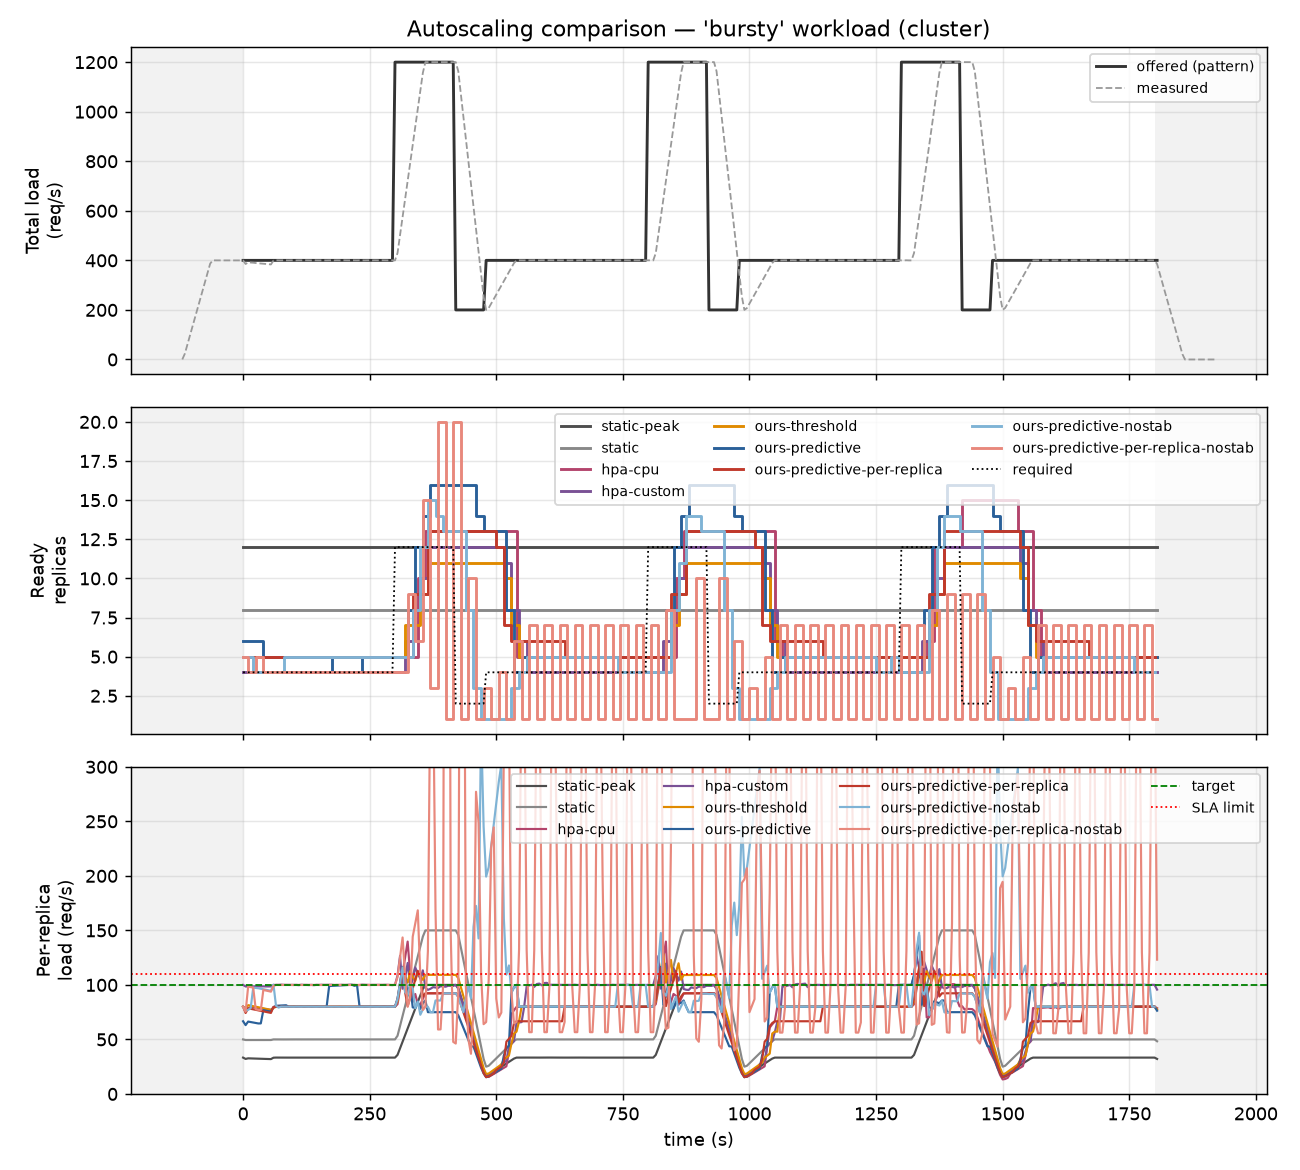
\includegraphics[width=\linewidth]{figures/comparison-bursty.png}
\caption[مقایسه‌ی بازوها روی بار کاری \lr{bursty}]{مقایسه‌ی بازوها روی \arm{bursty}.}
\label{fig:cmp-bursty}
\end{figure}

\textbf{\arm{hpa-cpu} خوب کار می‌کند و باید همین گفته شود.} روی \arm{ramp} و \arm{diurnal}
این بازو ۰/۰ درصد نقض دارد. یک شیب یکنوای آرام، بار کاری‌ای است که \lr{HPA} استاندارد از پس
آن برمی‌آید، و این نوشتار با گفتن آن قوی‌تر است تا با پنهان کردنش.

\subsection{زمان واکنش}
\label{sec:results-reaction}

مقایسه را روی \arm{diurnal} می‌آوریم، چون هر سه کنترل‌گر در آنجا واکنشی سنجیدنی دارند.

\begin{table}[H]
\centering
\caption{زمان واکنش میانه روی \arm{diurnal}}
\label{tab:results-reaction}
\begin{tabular}{|l|r|}
\hline
\textbf{بازو} & \textbf{زمان واکنش (میانه)} \\
\hline
\arm{hpa-custom} & ۱۱۲/۵ ثانیه \\
\arm{ours-threshold} & ۱۰۷/۵ ثانیه \\
\arm{hpa-cpu} & ۵۵/۰ ثانیه \\
\textbf{\arm{ours-predictive}} & \textbf{۲۷/۵ ثانیه} \\
\hline
\end{tabular}
\end{table}

سیاست پیش‌بینانه نزدیک به \textbf{چهار برابر} از \arm{hpa-custom} سریع‌تر است. هر دو دقیقاً
یک سنجه و یک نقطه‌ی هدف دارند. پس این تفاوت را نمی‌توان به کیفیت سنجه نسبت داد و تنها متغیر
باقی‌مانده سیاست است. همین شکل روی هر چهار الگو تکرار می‌شود: زمان واکنش
\arm{ours-predictive} میان ۲۰ تا ۳۵ ثانیه است در برابر ۳۲/۵ تا ۱۲۷/۵ ثانیه برای
\arm{hpa-custom}.

نکته‌ی دومی که ارزش گزارش دارد: \arm{hpa-custom} و \arm{ours-threshold} روی \arm{ramp}
عملاً \emph{بدل یکدیگرند} \mdash{} ۴/۷ در برابر ۴/۱ درصد نقض، ۱۲۷/۵ در برابر ۱۱۰/۰ ثانیه، و ۱۲،۰۴۰
در برابر ۱۱،۸۱۰ نمونه-ثانیه. دو کنترل‌گر واکنشی که مستقل از هم پیاده‌سازی شده‌اند و روی یک
سیگنال کار می‌کنند، در فاصله‌ی ۰/۶ واحد از هم می‌نشینند، که درون قدرت تفکیک اندازه‌گیری است.
این یعنی \textbf{خط مبنای واکنشی ما مثل نمونه‌ی استاندارد رفتار می‌کند}، پس سود پیش‌بینی،
مصنوعِ نوشتن یک رقیب ضعیف نیست.

\subsection{سربار خود مقیاس‌گذار}
\label{sec:results-overhead}

در یک اجرای واقعی، ۱۸ چرخه‌ی آشتی‌دهی مجموعاً ۰/۰۶۸ ثانیه زمان برد، یعنی حدود
\textbf{۳/۸ میلی‌ثانیه بر چرخه} در برابر فاصله‌ی ۱۵ ثانیه‌ای \mdash{} حدود ۰/۰۳ درصد. این عدد
نیازمندی غیرکارکردی «سربار منابع پایین» را برآورده می‌کند و هم‌زمان پرسش «آیا زمان واکنش
اندازه‌گیری‌شده‌ی شما صرفاً کندی کنترل‌گر خودتان نیست؟» را می‌بندد: زمان‌های واکنش
جدول~\ref{tab:results-reaction} از مرتبه‌ی ده‌ها ثانیه‌اند و زمان محاسبه‌ی کنترل‌گر از
مرتبه‌ی میلی‌ثانیه.

\section{آسیب‌شناسی پیش‌بینی بار هر نمونه}
\label{sec:results-perreplica}

یکی از یافته‌های مرکزی این پروژه در پیاده‌سازی به دست آمد و نه در طراحی. سازوکار آن در
بخش~\ref{sec:design-perreplica} توضیح داده شد. این بخش می‌پرسد که آیا آن سازوکار در خوشه‌ی
واقعی دیده می‌شود یا نه \mdash{} و پاسخ، ظریف‌تر از انتظار است.

جدول~\ref{tab:results-reversals} تعداد تغییر جهت را نشان می‌دهد. برای \arm{spike} و
\arm{bursty} سه تکرار مستقل انجام شد و ارقام جداگانه آمده است.

\begin{table}[H]
\centering
\caption{تعداد تغییر جهت؛ بازوی معیوب در برابر بازوی درست}
\label{tab:results-reversals}
\begin{tabular}{|l|l|l|}
\hline
\textbf{بار کاری} & \textbf{\arm{per-replica}} & \textbf{\arm{ours-predictive}} \\
\hline
\arm{ramp} & \lr{5} & \lr{0} \\
\arm{diurnal} & \lr{2} & \lr{2} \\
\arm{spike} & \lr{14, 4, 14} & \lr{3, 5, 7} \\
\arm{bursty} & \lr{10, 6, 5} & \lr{6, 7, 9} \\
\hline
\end{tabular}
\end{table}

نتیجه را باید با احتیاط خواند، و قاعده‌ی بخش~\ref{sec:method-repeatability} همین را ایجاب
می‌کند:

\begin{itemize}
  \item روی \arm{bursty} دو بازو کاملاً هم‌پوشانی دارند و بازوی معیوب حتی اندکی \emph{کمتر}
  نوسان می‌کند. این بار کاری آسیب‌شناسی را نشان نمی‌دهد و ادعای مربوط به آن پس گرفته می‌شود.
  \item روی \arm{spike} جدایی در دو اجرا از سه اجرا دیده می‌شود، اما یک اجرا با عدد ۴ درون
  دامنه‌ی بازوی سالم می‌افتد. شواهد در این شکل \emph{نشانه} است و نه نتیجه‌ی قطعی.
  \item روی \arm{diurnal} هیچ تفکیکی وجود ندارد: ۲ در برابر ۲.
  \item روی \arm{ramp} تفاوت روشن است \mdash{} ۵ در برابر صفر برای \emph{هر} بازوی دیگر.
\end{itemize}

از این تصویر یک نکته‌ی مکانیکی بیرون می‌آید که ارزش آن از خود اعداد بیشتر است. فرض اولیه این
بود که ناپایداری روی بارهایی ظاهر می‌شود که \emph{برمی‌گردند}. این فرض نادرست بود:
\arm{diurnal} برمی‌گردد و نوسان نمی‌کند، و \arm{ramp} هرگز برنمی‌گردد و نوسان می‌کند.

بیان دقیق‌تر آن است که \textbf{تحریک‌کننده‌ی ناپایداری، ناپیوستگی در ورودی یا در مشتق آن
است.} \arm{diurnal} برابر با $300 + 900\sin^2(\pi t / D)$ است و بی‌نهایت بار مشتق‌پذیر \mdash{} و
تنها الگویی است که آسیب‌شناسی در آن ظاهر نمی‌شود. \arm{spike} و \arm{bursty} توابع پله‌ای‌اند،
و \arm{ramp} پیوسته است اما در $t = 300$ و $t = 1500$ ناپیوستگی شیب دارد.

از این نکته یک هشدار عملی به دست می‌آید که مهم‌ترین پیام این بخش است:

\begin{quote}
\textbf{سیاستی که تنها روی یک بار کاری هموار سنجیده شود، پایدار به نظر می‌رسد بی‌آنکه باشد.}
روی \arm{diurnal} بازوی معیوب ۰/۰ درصد نقض دارد و از بازوی درست \emph{ارزان‌تر} هم هست
(۱۴،۹۱۵ در برابر ۱۵،۱۸۰ نمونه-ثانیه). هر کسی که اعتبارسنجی را روی یک منحنی هموار انجام دهد،
این سیاست را عرضه می‌کند.
\end{quote}

با این حال باید صادق بود: شواهد این بخش، به تنهایی، برای اثبات ادعا کافی نیست. اختلاف‌ها در
همان مرتبه‌ی پراکندگی خود بازوها هستند. آنچه ادعا را از این وضعیت ضعیف بیرون می‌آورد، آزمون
حذفی بخش بعد است.

\section{اثر سازوکار پایدارسازی: نتیجه‌ی اصلی}
\label{sec:results-stabilizer}

پرسش پژوهشی دوم این بود: سازوکار پایدارسازی چه مقدار نوسان را پنهان می‌کند و به چه بهایی؟
برای پاسخ، هر دو سیاست پیش‌بینانه یک بار دیگر اجرا شدند، این بار با
\lr{stabilization\_window\_seconds: 0}. یعنی میراگر برداشته شد و \emph{هیچ چیز دیگری} تغییر
نکرد. نتیجه در جدول~\ref{tab:results-nostab} آمده است.

\begin{table}[H]
\centering
\small
\caption{بازوهای حذفی: همان سیاست‌ها با میراگر خاموش}
\label{tab:results-nostab}
\begin{tabular}{|l|l|r|r|r|r|}
\hline
\textbf{بار کاری} & \textbf{بازو} & \textbf{نقض \lr{SLA}} & \textbf{نمونه-ثانیه} & \textbf{بالا/پایین} & \textbf{تغییر جهت} \\
\hline
\arm{spike} & \arm{per-replica-nostab} & \textbf{\lr{50.8\%}} & \lr{1,810} & \lr{60/60} & \textbf{\lr{119}} \\
\arm{spike} & \arm{predictive-nostab} & \lr{4.1\%} & \lr{12,355} & \lr{28/28} & \lr{43} \\
\arm{bursty} & \arm{per-replica-nostab} & \textbf{\lr{42.8\%}} & \lr{7,685} & \lr{49/50} & \textbf{\lr{98}} \\
\arm{bursty} & \arm{predictive-nostab} & \lr{13.0\%} & \lr{10,270} & \lr{27/23} & \lr{21} \\
\arm{ramp} & \arm{per-replica-nostab} & \textbf{\lr{39.5\%}} & \lr{7,360} & \lr{60/60} & \textbf{\lr{119}} \\
\arm{ramp} & \arm{predictive-nostab} & \lr{0.0\%} & \lr{13,395} & \lr{16/7} & \lr{12} \\
\hline
\end{tabular}
\end{table}

یک اجرای ۱۸۰۰ ثانیه‌ای با فاصله‌ی آشتی‌دهی ۱۵ ثانیه، ۱۲۰ چرخه‌ی کنترل دارد.
\textbf{عدد ۶۰ بالا و ۶۰ پایین یعنی کنترل‌گر در هر چرخه‌ی کنترل جهت خود را عوض می‌کند.} این
دیگر نوسان به معنای یک \emph{گرایش} نیست؛ نوسان به نقطه‌ی ثابت سامانه تبدیل شده است.

دو شاهد مستقل این تفسیر را تأیید می‌کنند:

\begin{enumerate}
  \item \textbf{فروپاشی ناوگان.} بازوی معیوب روی \arm{spike} تنها ۱،۸۱۰ نمونه-ثانیه مصرف
  می‌کند در برابر ۱۴،۲۸۰ برای بازوی درست. میانگین نمونه‌های آماده ۱/۰۰ روی \arm{spike}،
  ۴/۰۷ روی \arm{ramp} و ۴/۲۵ روی \arm{bursty} است. رقم \arm{spike} تیزترین بیان این شکست
  است: در سراسر پنجره‌ی ۱۸۰۰ ثانیه‌ای \textbf{شمار نمونه‌های آماده حتی یک بار هم از یک
  بالاتر نرفت}، حال آنکه \code{spec.replicas} تا ۱۱ بالا رفت و در ۱۲۰ حرکت (۶۰ بالا و ۶۰
  پایین) جابه‌جا شد. کنترل‌گر نمونه‌ها را سریع‌تر از آنکه بتوانند آماده شوند درخواست و لغو
  می‌کرد، پس هیچ نمونه‌ی تازه‌ای به خدمت نرسید (۱،۸۱۰ تقسیم بر ۱۸۰۰ برابر ۱/۰۱).
  \item \textbf{کم‌تأمین عظیم.} ۹،۶۲۰ نمونه-ثانیه کم‌تأمین روی \arm{spike}، در برابر ۲۷۰ برای
  بازوی درست.
\end{enumerate}

هر دو شاهد از کمیت‌هایی می‌آیند که مستقل از سری بار هر نمونه‌اند؛ محدودیتی که این سری در
همین سه اجرا دارد در بخش~\ref{sec:validity-metricdiff} ثبت شده است.

حال همین سیاست معیوب را با میراگر ۹۰ ثانیه‌ای بسنجید. روی \arm{ramp} نقض کیفیت خدمت برابر
۰/۰ درصد است و روی \arm{spike} برابر ۰/۶ درصد. یعنی \emph{از همه‌ی آزمون‌های کیفیت و هزینه‌ی
این فصل سربلند بیرون می‌آید}.

نتیجه‌ی اصلی این پایان‌نامه از همین‌جا می‌آید:

\begin{quote}
\textbf{یک پنجره‌ی پایدارسازی ۹۰ ثانیه‌ای می‌تواند یک قانون کنترل بنیاداً معیوب را چنان
بپوشاند که از همه‌ی آزمون‌های کیفیت خدمت و هزینه سربلند بیرون بیاید.}
\end{quote}

این ادعا سه برتری بر شکل اولیه‌ی خود \mdash{} یعنی شمارش تغییر جهت در بخش~\ref{sec:results-perreplica}
\mdash{} دارد. نخست آنکه بزرگی اثر نزدیک به \emph{ده برابر} پراکندگی اندازه‌گیری است و نه درون آن:
۱۱۹ تغییر جهت در برابر ۱۲، و ۵۰/۸ درصد در برابر ۴/۱ درصد. دوم آنکه به شمارش در یک اجرای منفرد
تکیه ندارد و روی هر سه الگوی ناهموار تکرار می‌شود. سوم آنکه \emph{توضیح می‌دهد} چرا سیاست
معیوب روی \arm{diurnal} سالم به نظر می‌رسید: میراگر کار را می‌کرد، و یک بار کاری هموار فشار
چندانی به آن نمی‌آورد.

برای مهندس سامانه نتیجه‌ی عملی روشن است:

\begin{quote}
\textbf{ارزیابی پایداری باید میراگر را خاموش کند و بار کاری پله‌ای بدهد.} وگرنه چیزی را
می‌سنجد که پیشاپیش پنهان شده است.
\end{quote}

توجه شود که این ادعا درباره‌ی \emph{بی‌فایده بودن} میراگر نیست. میراگر کار خودش را به‌خوبی
انجام می‌دهد و بازوی \arm{ours-predictive} نیز به آن نیاز دارد: بدون آن، همان سیاست \emph{درست}
هم روی \arm{bursty} از ۱/۱ به ۱۳/۰ درصد نقض می‌رسد. ادعا این است که میراگر یک
\emph{اصلاح} نیست، و ارزیابی‌ای که آن را روشن نگه دارد نمی‌تواند سالم را از معیوبِ میراشده
تفکیک کند.

\section{مقایسه با شبیه‌ساز}
\label{sec:results-simulator}

برای اعتبارسنجی متقابل، \emph{ترتیب} بازوها در شبیه‌ساز و در خوشه مقایسه شد. مقایسه روی ترتیب
است و نه مقدار مطلق، چون شبیه‌ساز شبکه ندارد و تأخیر راه‌اندازی را ساده مدل می‌کند؛ انتظار
هم‌خوانی مقادیر از ابتدا وجود نداشت.

از هشت ترتیب قابل مقایسه، \textbf{پنج مورد توافق دارند}. هر سه اختلاف روی بارهای کاری
\emph{پله‌ای} رخ داده \mdash{} یعنی \arm{spike} و \arm{bursty} \mdash{} و همگی در یک جهت‌اند: شبیه‌ساز
سیاست واکنشی را جلوتر از سیاست پیش‌بینانه رتبه می‌دهد و خوشه عکس آن را می‌گوید.

علت محتمل روشن است و به بخش~\ref{sec:bg-measurement-lag} برمی‌گردد. شبیه‌ساز بی‌درنگ مقیاس به
پایین می‌دهد و هیچ تأخیر اندازه‌گیری ندارد؛ بار هر نمونه را دقیقاً و بی‌واسطه حساب می‌کند.
خوشه اما پیش از دیدن هر تغییر، یک فاصله‌ی جمع‌آوری به‌علاوه‌ی یک پنجره‌ی یک‌دقیقه‌ای
\lr{rate} هزینه می‌کند. \textbf{تأخیر اندازه‌گیری دقیقاً همان چیزی است که پیش‌بینی جبرانش
می‌کند}، پس حذف آن از مدل، به سود بازوی واکنشی تمام می‌شود.

نتیجه‌ی عملی محدود و مشخص است: شبیه‌ساز برای استدلال درباره‌ی پیکربندی‌ها روی بارهای هموار
قابل اتکاست، اما ترتیب آن روی بارهای پله‌ای قابل اعتماد نیست و هر نتیجه‌ای از آنجا به وارسی
نقطه‌ای روی خوشه نیاز دارد.

\section{تکرارپذیری و قدرت تفکیک}
\label{sec:results-repeatability}

جدول~\ref{tab:results-repeat} نتیجه‌ی تکرارها را نشان می‌دهد. مقادیر به‌جای میانگین‌گیری
تک‌تک آمده‌اند.

\begin{table}[H]
\centering
\small
\caption{اجراهای مستقل تکراری؛ هر مقدار یک اجرای جداگانه است}
\label{tab:results-repeat}
\begin{tabular}{|l|l|l|l|l|}
\hline
\textbf{بار کاری} & \textbf{بازو} & \textbf{نقض \lr{SLA}} & \textbf{نمونه-ثانیه} & \textbf{تغییر جهت} \\
\hline
\arm{spike} & \arm{ours-predictive} & \lr{0.3, 0.8, 0.6} & \lr{14,085 / 14,350 / 14,280} & \lr{3, 5, 7} \\
\arm{spike} & \arm{ours-pred.-per-replica} & \lr{0.8, 0.6, 0.6} & \lr{13,900 / 14,030 / 13,900} & \lr{14, 4, 14} \\
\arm{bursty} & \arm{ours-predictive} & \lr{0.8, 0.3, 1.1} & \lr{14,545 / 14,545 / 14,385} & \lr{6, 7, 9} \\
\arm{bursty} & \arm{ours-pred.-per-replica} & \lr{2.5, 2.2, 1.9} & \lr{13,715 / 13,760 / 13,465} & \lr{10, 6, 5} \\
\arm{ramp} & \arm{ours-threshold} & \lr{5.2, 4.1} & \lr{12,050 / 11,810} & \lr{0, 0} \\
\arm{ramp} & \arm{static} & \lr{35.5, 35.6} & \lr{14,440 / 14,480} & \lr{0, 0} \\
\arm{spike} & \arm{hpa-custom}$^{\dagger}$ & \lr{2.8, 2.8} & \lr{17,105 / 17,055} & \lr{0, 0} \\
\hline
\end{tabular}
\end{table}

\noindent$^{\dagger}$ این دو اجرا \emph{پیش از} اصلاح تحویل بار
(بخش~\ref{sec:results-loaddefect}) انجام شده‌اند و به همین دلیل با سطر \arm{hpa-custom} در
جدول~\ref{tab:results-headline} \mdash{} که از اندازه‌گیری مجدد می‌آید \mdash{} قابل مقایسه نیستند. اینجا
تنها به‌عنوان یک جفت تکرار \emph{هم‌شرایط با یکدیگر} آورده شده‌اند. گروه‌بندی تکرارها بر
پایه‌ی شرایط اجرا و نه صرفاً نام بازو، همان نکته‌ای است که
بخش~\ref{sec:method-repeatability} بر آن تأکید کرد: اگر این دو با اجراهای پس از اصلاح در یک
گروه ریخته می‌شدند، فاصله‌ی میان دو \emph{آزمایش} به‌عنوان نویز \emph{این بازو} گزارش می‌شد و
پراکندگی متورم، یافته‌های واقعی را رد صلاحیت می‌کرد.

سه عدد از این جدول بیرون می‌آید که قدرت تفکیک کل ارزیابی را تعیین می‌کنند:

\begin{itemize}
  \item پراکندگی نمونه-ثانیه برای اجراهای هم‌شرایط میان \textbf{۴۰ تا ۲۹۵} است، یعنی حدود دو
  درصد.
  \item بازوی بدون کنترل‌گر (\arm{static}) تا ۰/۱ درصد بازتولید می‌شود؛ بازوهای خودکار حدود
  یک واحد درصد تغییر می‌کنند. این تفاوت میان اندازه‌گیری یک حلقه‌ی \emph{باز} و یک حلقه‌ی
  \emph{بسته} است.
  \item بنابراین \textbf{تفاوت‌های کمتر از حدود ۱/۵ واحد درصد در نقض کیفیت خدمت میان دو بازوی
  خودکار، در $n=1$ قابل تفکیک نیستند.}
\end{itemize}

بر پایه‌ی همین قاعده بود که در بخش~\ref{sec:results-perreplica} ادعای مربوط به \arm{bursty}
پس گرفته شد و ادعای \arm{spike} به نشانه تنزل یافت. در مقابل، اثر سازوکار پایدارسازی در
بخش~\ref{sec:results-stabilizer} نزدیک به ده برابر این پراکندگی است و به‌راحتی از آن عبور
می‌کند. همین است که آن را به نتیجه‌ی اصلی تبدیل می‌کند و نه یک مشاهده‌ی جالب.

\section{محدودیت‌های اعتبار}
\label{sec:results-validity}

این بخش عمداً مفصل است.

\subsection{تأخیر در این آزمایش تفکیک‌کننده نیست}
\label{sec:results-latency}

«تأخیر پاسخ به کاربر در زمان جهش» یکی از سنجه‌های مقایسه بود. این سنجه در
عمل میان بازوها هیچ تفاوتی نشان نمی‌دهد \mdash{} ستون صدک ۹۵ در هر بازو و هر الگوی بار میان ۲/۴ و ۲/۵
میلی‌ثانیه است \mdash{} و اکنون دلیلش را دقیق می‌دانیم.

محدودیت پردازنده‌ی کانتینر روی این میزبان \emph{اعمال نمی‌شود}. نمونه در بار ۲۲۰۰ درخواست بر
ثانیه ۳/۶۵ هسته مصرف می‌کند حال آنکه \lr{limits.cpu} برابر ۱ است، و شمارنده‌ی دوره‌های
گلوگاه‌شده‌ی زمان‌بند دقیقاً \emph{صفر} می‌ماند. متغیر \lr{GOMAXPROCS} نیز تنظیم نشده، پس
زمان اجرای \lr{Go} هر ۱۴ هسته‌ی گره را می‌بیند. یک نمونه‌ی گرم، ۲۲۰۰ درخواست بر ثانیه را با
صدک ۹۵ برابر ۳/۳۴ میلی‌ثانیه و بدون خطا سرویس می‌دهد.

پس ظرفیت واقعی هر نمونه بیش از ۲۲۰۰ درخواست بر ثانیه است، در برابر نرخ هدف ۱۰۰ \mdash{} یعنی بیش از
بیست برابر. هیچ بازویی در این ارزیابی حتی به یک مرتبه‌ی بزرگی اشباع نزدیک نمی‌شود.

\textbf{عدد ۲/۴ میلی‌ثانیه خطا نیست؛ اندازه‌گیری درستی است که تفکیک نمی‌کند.} تکرار
آزمایش‌ها ستون یکسانی تولید می‌کرد، پس اجرای دوباره برای «به دست آوردن تأخیر واقعی» بی‌فایده
است.

با این حال می‌توان نشان داد که سنجه‌ی تأخیر سالم است و به تأمین منابع پاسخ می‌دهد. تعداد
نمونه تثبیت شد و بار ثابت ۸۰۰ درخواست بر ثانیه داده شد
(جدول~\ref{tab:results-latency-pinned}):

\begin{table}[H]
\centering
\caption{پاسخ تأخیر به تأمین منابع، با ناوگان تثبیت‌شده و بار ثابت ۸۰۰ درخواست بر ثانیه}
\label{tab:results-latency-pinned}
\begin{tabular}{|r|r|r|r|}
\hline
\textbf{نمونه‌ها} & \textbf{تحویل‌شده} & \textbf{تأخیر صدک ۹۵} & \textbf{خطا} \\
\hline
۱ & \lr{792.9} & \textbf{\lr{2276 ms}} & \lr{5.05\%} \\
۲ & \lr{800.6} & \textbf{\lr{2.59 ms}} & \lr{0\%} \\
۴ & \lr{800.0} & \lr{2.60 ms} & \lr{0\%} \\
۸ & \lr{800.0} & \lr{2.65 ms} & \lr{0\%} \\
\hline
\end{tabular}
\end{table}

افزودن \emph{یک} نمونه دُم توزیع تأخیر را نزدیک به ۸۸۰ برابر بهبود می‌دهد. این دو چیز را
نشان می‌دهد: نخست آنکه افزودن نمونه واقعاً ترافیک بیشتری را سرویس می‌دهد \mdash{} که تا پیش از این
آزمایش، هیچ شاهد \emph{فیزیکی} برای آن در داده‌های ارزیابی وجود نداشت \mdash{} و دوم آنکه سنجه‌ی
تأخیر سالم است و فقط در بازه‌ی بار این آزمایش اشباع نشده.

نتیجه‌ی روش‌شناختی روشن است: \textbf{تأخیر در این پایان‌نامه به‌عنوان نتیجه‌ی کالیبراسیون
گزارش می‌شود و نه به‌عنوان سنجه‌ی مقایسه‌ی بازوها.}

\subsection{سنجه‌ی نقض کیفیت خدمت چه چیزی را می‌سنجد}
\label{sec:results-slameaning}

«نقض \lr{SLA}» در این فصل سنجه‌ی \textbf{رزرو ظرفیت} است و نه
سنجه‌ی \textbf{آسیب کاربر}. این سنجه می‌پرسد آیا ناوگان چنان اندازه‌گذاری شده که بار هر نمونه
درون درخواست تضمین‌شده‌ی پردازنده بماند.

این پرسش، پرسش درست و متعارف ظرفیت‌سنجی است، چون ظرفیت مازاد تنها تا وقتی در دسترس است که گره
خلوت باشد و این گره اختصاصی است. اما رقم ۴۰ درصدی نقض به این معنا نیست که کاربران چیزی
دیده‌اند؛ در این آزمایش‌ها ندیده‌اند.

\subsection{نقص تحویل بار}
\label{sec:results-loaddefect}

جدی‌ترین نقص اندازه‌گیری کشف‌شده در این پروژه، و موردی که از تمام بررسی‌های خودکار
بخش~\ref{sec:method-validity} گذشت.

مولد بار به‌صورت پیش‌فرض از اتصال پایدار \lr{HTTP} استفاده می‌کرد. هر کاربر مجازی یک اتصال
\lr{TCP} برای تمام عمرش نگه می‌دارد، و هر اتصال به همان نمونه‌ای سنجاق می‌شود که
\lr{kube-proxy} هنگام باز شدن آن انتخاب کرده است. چون برنامه در حدود ۲/۴ میلی‌ثانیه پاسخ
می‌دهد، سناریوی نرخ‌محور هرگز به بیش از چند کاربر مجازی هم‌زمان نیاز پیدا نکرد \mdash{} و چند کاربر
مجازی یعنی چند اتصال یعنی چند نمونه. جدول~\ref{tab:results-connfix} اثر را مستقیماً نشان
می‌دهد.

\begin{table}[H]
\centering
\caption{آزمون \lr{A/B} کنترل‌شده در ۸۰۰ درخواست بر ثانیه در برابر ۸ نمونه}
\label{tab:results-connfix}
\begin{tabular}{|l|c|r|r|}
\hline
\textbf{مدل اتصال} & \textbf{نمونه‌های سرویس‌دهنده} & \textbf{تحویل‌شده} & \textbf{تأخیر صدک ۹۵} \\
\hline
اتصال پایدار (پیش‌فرض) & \textbf{۱ از ۸} & \lr{508/800} & \textbf{\lr{1.5 s}} \\
اتصال به ازای هر درخواست & \textbf{۷ از ۸} & \lr{800/800} & \lr{2.71 ms} \\
\hline
\end{tabular}
\end{table}

هیچ چیزی در چارچوب این را گزارش نکرد، چون مولد بار نرخ کامل درخواست‌شده را تحویل می‌داد و هر
درخواست هم کد ۲۰۰ برمی‌گرداند.

\textbf{گستره‌ی آسیب اندازه‌گیری شد و به فرض بسنده نشد.} ورودی خود مقیاس‌گذار، چنان‌که در
بخش~\ref{sec:design-collector} آمد، حاصل تقسیم \emph{مجموع} \lr{rate} روی همه‌ی سری‌ها بر
\emph{شمارش} نمونه‌های آماده است و به اینکه کدام نمونه سرویس داده وابسته نیست. هر دو طرف
مستقیماً در میانه‌ی یک اجرا پرس‌وجو شدند: صورت ۱۲۹۹/۹۹ و مخرج ۱۳، یعنی هر دو درست.

اما این استدلال یک حفره دارد: اگر نمونه‌های سنجاق‌شده اشباع می‌شدند، صورت کسر دیگر بار مورد
نظر آزمایش نبود بلکه هر چیزی بود که آن چند نمونه می‌توانستند جذب کنند. پس بار تحویل‌شده در
\emph{تمام ۴۵ اجرای موجود در زمان این بررسی} \mdash{} یعنی ۴۹ اجرای معتبر منهای چهار
اندازه‌گیری مجدد \arm{hpa-custom} که هنوز انجام نشده بود \mdash{} با انتگرال الگو مقابله شد:

\begin{quote}
\textbf{۴۲ اجرا از ۴۵ اجرا در بازه‌ی ۰/۹۹۳ تا ۱/۰۱۰ از مقدار هدف قرار گرفتند.}
\end{quote}

دلیلش ساده است: سه یا چهار نمونه‌ی برنامه‌ای با پاسخ ۲/۴ میلی‌ثانیه‌ای حدود ۱۵۰۰ درخواست بر
ثانیه جذب می‌کنند، که بالاتر از اوج هر الگو در این مجموعه است. بار عرضه‌شده هرگز خفه نشد.

سه استثنا همگی به بازوی \arm{per-replica-nostab} تعلق دارند (نسبت‌های ۰/۳۸۵، ۰/۴۰۹ و ۰/۴۱۳).
این بازو ناوگان خود را فروپاشانده بود، و آنچه کم تحویل شد \emph{خود نتیجه} است و نه نقص
اندازه‌گیری \mdash{} و اگر اثری داشته باشد، ارقام نقض ۳۹ تا ۵۱ درصدی را \emph{محافظه‌کارانه}
می‌کند، چون صورت خفه‌شده مقدار نقض را کم‌برآورد می‌کند.

دو سنجه‌ی متفاوت در کارند و نباید با هم اشتباه شوند: نسبت‌های بالا \emph{سمت ناوگان} را
می‌سنجند (مقدار \code{sum(rate(...))} که واقعاً به برنامه رسید، درون فلات‌های دست‌کم ۱۵۰
ثانیه‌ای)، حال آنکه دروازه‌ی خودکار بخش~\ref{sec:method-validity} شمارش \code{http\_reqs}
خود \lr{k6} را می‌سنجد و روی همین سه اجرا ۰/۹۹۹ و ۰/۹۸۸ و ۰/۹۹۹ گزارش می‌کند. \lr{k6}
تقریباً همه‌ی درخواست‌ها را \emph{فرستاد}؛ ناوگان فروپاشیده تنها بخشی را \emph{سرویس داد}.

ظرفیت یک نمونه هم در دو رژیم اندازه گرفته شده: رقم ۲۲۰۰ درخواست بر ثانیه‌ی
بخش~\ref{sec:results-latency} از یک نمونه‌ی گرم و اختصاصی با مدل اتصال اصلاح‌شده می‌آید،
حال آنکه این سه اجرا پیش از اصلاح و با نمونه‌ای در حال ساخته و نابود شدن انجام شده‌اند
(میانگین بار سرویس‌شده روی \arm{spike} برابر ۳۶۸/۹ درخواست بر ثانیه).

بنابراین نقض کیفیت خدمت، نمونه-ثانیه، کم‌تأمین و بیش‌تأمین، و شمارش تغییر جهت دست‌نخورده
ماندند. آنچه باطل شد دو چیز بود: ستون تأخیر \mdash{} که طبق بخش~\ref{sec:results-latency} به‌هرحال
تفکیک‌کننده نیست \mdash{} و بازوی \arm{hpa-custom} که تنها مصرف‌کننده‌ی سنجه‌ی \emph{هر نمونه} است.
آن بازو روی هر چهار بار کاری از نو اندازه‌گیری شد و همه‌ی ارقام \arm{hpa-custom} در این فصل
از اجرای تازه می‌آید.

دامنه‌ی این اصلاح باید صریح باشد: تنها \textbf{۴ اجرا از ۴۹ اجرای معتبر} زیر قرارداد
اصلاح‌شده گرفته شده‌اند و هر چهار همین اندازه‌گیری‌های \arm{hpa-custom} هستند. ۴۵ اجرای
دیگر \mdash{} از جمله همه‌ی سطرهای جدول~\ref{tab:results-nostab} \mdash{} پیش از اصلاح‌اند و
مجوزشان همان بررسی گستره‌ی آسیب بالاست. میدان \code{load\_contract} در \code{run.json} هر
اجرا این تفکیک را ثبت می‌کند.

\subsection{نتیجه‌ای که با اندازه‌گیری مجدد پس گرفته شد}
\label{sec:results-hpacustom-redo}

اندازه‌گیری مجدد \arm{hpa-custom} یک ادعای پیشین را باطل کرد. صداقت گزارش ایجاب می‌کند که ثبت
شود.

پیش از اصلاح، این بازو روی هیچ بار کاری مقیاس به پایین نمی‌داد و گران‌ترین بازوی خودکار بود.
پس از اصلاح (جدول~\ref{tab:results-hpacustom}):

\begin{table}[H]
\centering
\caption{اثر اصلاح تحویل بار بر بازوی \arm{hpa-custom}}
\label{tab:results-hpacustom}
\begin{tabular}{|l|l|l|r|}
\hline
\textbf{بار کاری} & \textbf{مقیاس به پایین} & \textbf{نمونه-ثانیه} & \textbf{تغییر} \\
\hline
\arm{ramp} & \lr{2 $\rightarrow$ 3} & \lr{12,025 $\rightarrow$ 12,040} & \textbf{‎+۰/۱ درصد} \\
\arm{diurnal} & \lr{1 $\rightarrow$ 11} & \lr{17,115 $\rightarrow$ 14,365} & -۱۶ درصد \\
\arm{spike} & \lr{0--1 $\rightarrow$ 7} & \lr{17,055 $\rightarrow$ 12,255} & -۲۸ درصد \\
\arm{bursty} & \lr{1 $\rightarrow$ 14} & \lr{18,980 $\rightarrow$ 11,965} & -۳۷ درصد \\
\hline
\end{tabular}
\end{table}

سازوکار نیز تأیید شد و صرفاً حدس نماند. قاعده‌ی سنجه‌های غایب \lr{HPA}
(بخش~\ref{sec:bg-hpa}) فرض می‌کند نمونه‌هایی که سنجه ندارند در نقطه‌ی هدف‌اند، و این فرض
\emph{تنها} مسیر مقیاس به پایین را می‌بندد. اگر این سازوکار درست باشد، نقص نباید روی یک بار
کاری \emph{یکنوا} اثری بگذارد. \arm{ramp} تنها بار یکنوای مجموعه است و به اندازه‌ی ۰/۱ درصد
تغییر کرد، در حالی که هر سه بار دیگر به‌شدت جابه‌جا شدند. اثر دقیقاً جایی ظاهر شد که سازوکار
پیش‌بینی می‌کند و جای دیگری ظاهر نشد.

پس ادعای «\lr{HPA} روی سنجه‌ی سفارشی هرگز مقیاس به پایین نمی‌دهد» \textbf{پس گرفته می‌شود}؛
آن رفتار مصنوع مولد بار بود و نه ویژگی سنجه‌های سفارشی.

این اصلاح ادعای خود پروژه را هم جابه‌جا می‌کند. پیش از آن، بازوی
\arm{ours-predictive} روی \arm{diurnal} در هر سه محور هم‌زمان بر \arm{hpa-custom} برتری
داشت. پس از اصلاح، بازوی ما در کیفیت خدمت پیش است (۰/۰ در برابر ۴/۷ درصد) و در زمان واکنش نیز
(۲۷/۵ در برابر ۱۱۲/۵ ثانیه)، اما \textbf{در هزینه ۵/۷ درصد عقب می‌افتد}. همین شکل روی هر
چهار بار کاری تکرار می‌شود.

پس ادعای قابل دفاع همان \emph{مبادله}‌ی بخش~\ref{sec:results-headline} است و نه برتری هم‌زمان
در هر سه محور.

این مورد یک درس روش‌شناختی هم دارد که ارزش آن از خود عدد بیشتر است:
\textbf{یک بازوی مقایسه‌ی معیوب، بازوی خودی را رایگان جلوه می‌دهد.} آزمون حذفی دقیقاً برای
گرفتن همین حالت وجود دارد، و در اینجا تنها به این دلیل کار کرد که آن بازو دوباره اجرا شد و
به آن اعتماد نشد.

\subsection{تفاوت تصویر اجراشده با کد مخزن}
\label{sec:results-image}

اندازه‌گیری‌ها روی تصویری از برنامه‌ی نمونه انجام شد که از روی کد نهایی مخزن ساخته‌شدنی نیست.
بررسی مستقیم نقطه‌ی \lr{/metrics} یک نمونه‌ی در حال اجرا نشان می‌دهد شمارنده‌ی
\code{http\_requests\_shed\_total} در آن وجود ندارد، در حالی که
\code{http\_requests\_in\_flight} هست. پس محتوای آن مقدم بر افزودن سازوکار محدودسازی هم‌زمانی
است. دو پیامد دارد:

\begin{itemize}
  \item \textbf{سنجه‌ی «درخواست‌های ریخته‌شده» در هر ۴۹ اجرا ساختاراً نابینا بوده است.} صفر
  بودنش به معنای رخ‌ندادن نیست، به معنای \emph{نبودن سنجه} است. هر خوانشی از داده‌های این
  پروژه به شکل «هیچ درخواستی ریخته نشد» بی‌پشتوانه است.
  \item \textbf{محدودکننده‌ی ۱۶ درخواست هم‌زمان فعال نبوده است.} در بازوهای
  \arm{per-replica-nostab} شمارش درخواست‌های در جریان روی یک نمونه به ۶۱ رسیده که تنها با
  هم‌زمانی نامحدود ممکن است.
\end{itemize}

در جریان ردیابی این موضوع یک درس عمومی هم به دست آمد:
\textbf{یک برچسب، یک هویت نیست.} انبار تصاویر میزبان و انبار تصاویر گره، دو تصویر
\emph{متفاوت} را زیر یک برچسب یکسان نگه داشته بودند. تنها مرجع قابل اتکا برای اینکه
\lr{kubelet} چه چیزی را اجرا کرده، اثرانگشت ثبت‌شده در وضعیت خود نمونه است.

تصمیم گرفته شد تصویر تثبیت و مستند شود و بازسازی نشود. دلیلش این است که بازسازی، ریختن
درخواست‌ها با کد ۵۰۳ را بالای ۱۶ درخواست هم‌زمان فعال می‌کند و رفتار فیزیکی همه‌ی بازوها را
تغییر می‌دهد \mdash{} به‌ویژه بازوهای فروپاشیده که به ۶۱ رسیده بودند. یعنی آزمایشی \emph{متفاوت}
می‌شود و نه اصلاحی جزئی، و هیچ‌یک از ۴۹ اجرای موجود با آن قابل مقایسه نمی‌ماند. هر ۴۹ اجرا
روی همین یک تصویر انجام شده‌اند، پس نسبت به یکدیگر کاملاً قابل مقایسه‌اند. چارچوب آزمایش اکنون
اثرانگشت را پیش از هر اجرا مقابله می‌کند، اجرایی را که ناوگانش بیش از یک اثرانگشت داشته باشد
رد می‌کند، و اثرانگشت را در فراداده‌ی هر اجرا ثبت می‌کند.

آشتی دادن تصویر و کد مخزن، کاری برای پس از این نوشتار است.

\subsection{هشدار واگرایی سنجه}
\label{sec:validity-metricdiff}

تحلیل‌گر بررسی می‌کند که سری \code{autoscaler\_metric\_value} گزارش‌شده توسط مقیاس‌گذار با
سری \code{per\_replica\_rps} که تحلیل مستقلاً می‌گیرد بخواند، و روی سه اجرای
\arm{per-replica-nostab} اختلاف ۸۶ تا ۱۳۵ درصد گزارش می‌کند. این دو، \emph{یک عبارت
\lr{PromQL} یکسان}‌اند و پس‌خور هر دو را به یک اندازه جابه‌جا می‌کند؛ پس اختلافشان اختلاف
زمان نمونه‌برداری است \mdash{} مقیاس‌گذار روی چرخه‌ی ۱۵ ثانیه‌ای و تحلیل روی شبکه‌ی ۵
ثانیه‌ای، با مخرج \code{count(up)} که میان دو قرائت جابه‌جا می‌شود. معنای این هشدار آن است
که بازسازی تحلیل از سیگنال لزوماً همان چیزی نیست که سیاست بر اساس آن تصمیم گرفته. ارقام
بخش~\ref{sec:results-stabilizer} از آن متأثر نیستند، چون بر شمارش تغییر جهت روی
\code{spec.replicas} و بر نمونه-ثانیه استوارند و هیچ‌کدام از این سری مشتق نمی‌شوند.

\subsection{سایر محدودیت‌ها}
\label{sec:results-otherlimits}

\textbf{تک‌گره و بدون رقابت.} خوشه یک گره اختصاصی ۱۴ هسته‌ای است. ظرفیت مازادی که در
بخش~\ref{sec:results-latency} دیده شد، روی گره‌ای که با سرویس‌های دیگر مشترک باشد در دسترس
نخواهد بود. نتایج به خوشه‌های چندمستأجری تعمیم‌پذیر نیستند بدون اندازه‌گیری دوباره.

\textbf{تعداد تکرار.} تنها چند بازو سه بار تکرار شده‌اند. نتایجی که به تفاوت‌های کوچک وابسته
بودند در این فصل به‌عنوان نشانه گزارش شده‌اند و نه نتیجه.

\textbf{یک سرویس، بدون‌حالت.} هیچ زنجیره‌ی چندسرویسی آزموده نشده است. در چنین زنجیره‌ای،
مقیاس‌گیری یک سرویس بار سرویس بعدی را تغییر می‌دهد و مسیر پس‌خور تازه‌ای می‌سازد که این
ارزیابی آن را نمی‌بیند.

\textbf{اثر رگبار سرد.} نخستین رگبار بار روی یک نمونه‌ی سرد تأخیر صدک ۹۵ حدود ۲/۵ ثانیه و ۱۳
تا ۲۶ درصد خطا نشان می‌دهد، در حالی که همان نمونه در حالت گرم چنین رفتاری ندارد. این حالت پس
از حدود سه دقیقه بی‌کاری بازمی‌گردد، پس گذرای مقیاس به پایین نیست. سازوکارش هنوز روشن نیست.
هر اجرای اندازه‌گیری‌شده با مرحله‌ی گرم‌کردن آغاز می‌شود، پس نتایج این فصل از آن متأثر
نیستند. با این حال این پدیده ممکن است سود پیش‌بینی را از راهی توضیح دهد که سنجه‌های فعلی
نمی‌بینند \mdash{} نمونه‌ای که \emph{پیش از} رسیدن بار افزوده شود گرم است، و نمونه‌ای که واکنشی
افزوده شود سرد \mdash{} و برای کار آینده پیشنهاد می‌شود.

\section{جمع‌بندی فصل}
\label{sec:results-summary}

\textbf{درباره‌ی کارایی.} در میان بازوهای خودکار، سیاست پیش‌بینانه روی هر چهار بار کاری
کم‌ترین کم‌تأمین منابع را دارد و نقض کیفیت خدمتش کم‌ترین یا هم‌تراز کم‌ترین است، و زمان
واکنشش روی \arm{diurnal} نزدیک به چهار برابر بهتر از
\arm{hpa-custom} است که همان سیگنال و همان نقطه‌ی هدف را دارد. اما این برتری به بهای ۵/۷ تا ۲۰/۲
درصد ظرفیت بیشتر به دست می‌آید. \textbf{ادعای درست یک مبادله است و نه برتری مطلق.}

\textbf{درباره‌ی پایداری.} پیش‌بینی بار هر نمونه به‌جای بار کل، حلقه‌ی کنترل را ناپایدار
می‌کند. با میراگر روشن، این ناپایداری در سنجه‌های متعارف تقریباً دیده نمی‌شود و روی یک بار
کاری هموار اصلاً دیده نمی‌شود.

\textbf{نتیجه‌ی اصلی.} با خاموش کردن میراگر، همان سیاست تا ۵۰/۸ درصد نقض کیفیت خدمت و ۱۱۹
تغییر جهت در ۱۲۰ چرخه‌ی کنترل می‌رسد. پس یک پنجره‌ی پایدارسازی ۹۰ ثانیه‌ای می‌تواند یک قانون
کنترل معیوب را چنان بپوشاند که از همه‌ی آزمون‌ها سربلند بیرون بیاید. \textbf{ارزیابی پایداری
باید میراگر را خاموش کند و بار کاری پله‌ای بدهد.}

\textbf{درباره‌ی اعتبار.} تأخیر در بازه‌ی بار این آزمایش تفکیک‌کننده نیست و به‌عنوان نتیجه‌ی
کالیبراسیون گزارش شده است. سنجه‌ی نقض کیفیت خدمت سنجه‌ی رزرو ظرفیت است و نه سنجه‌ی آسیب
کاربر. یک نقص تحویل بار کشف و اندازه‌گیری شد و بازوی آسیب‌دیده از نو اجرا شد، که به پس گرفتن
یکی از قوی‌ترین ادعاهای پیشین انجامید. و تصویر اندازه‌گیری‌شده از کد مخزن ساخته‌شدنی نیست،
که ثبت شده و تثبیت شده است.
